\documentclass[../main.tex]{subfiles}

\begin{document}

\section{What language? What grammar?}

This proto-book is about aspects of the grammar of the contemporary Chinese language (现代汉语). 
Each word in this phrase can trigger controversy. Before we start substantial discussion, it is a wise idea 
to clarify what we are actually talking about. 

\subsection{Standard Mandarin and its variation}

% 新文化运动时期的作品读着不顺口

In the rest of the proto-book, we use the term \emph{Chinese} 中文,(现代)汉语,华语 interchangeably with 
the more precise term \emph{Standard Mandarin Chinese}.

\subsection{The possibility to have a structure-based grammar}\label{sec:structure-based}

People familiar with Chinese often say its grammar depends more on the context, and some goes as far as 
claiming that a structure-based approach -- or even a truth-value semantics-based approach -- is infeasible 
when studying Chinese. And indeed, \citet{li1989mandarin}, arguably the most recognized grammar of the Chinese 
language, is a functionalist one. Our opinion is that though of course the context can influence strongly the 
grammar, this is not without limit. Pragmatic information may trigger \emph{pro}-drop or forbid it, but it 
rarely triggers omission of the object. Sentences in dialogues may have more sentence final particles than 
written ones, but spoken sentences never have sentence \emph{initial} particles. Though the context means 
a lot in Chinese, it is safe to assume we still have an underlying rigid structure beside purely semantic 
or pragmatic information.

The structure-based approach is by no means a rejection of functionalist studies. Rather, the former explores 
what features can be employed by the latter, so it can be expected the two approaches are complementary.

The next question is how to catch the structure. It is impossible to sit there and just ``observe the world without bias''. People always do observation within a 
framework. Some may argue that typologists must be ready to invent completely new concepts when documenting 
a language (see, for example, \citet{haspelmath2008framework}), which is, of course, in principle true, 
but practically it is common for people to implicitly take some concepts for granted and carry out 
valuable works. R.M.W Dixon, a famous opponent of generative syntax, mocks ``formalists'' who fruitlessly try 
to find concepts exact corresponding to Indo-European ones in underdocumented languages in his 
\ac{blt} \citep{dixon2009basic} and advocates ``describing a language in its own terms'',
but he immediately goes on to discuss how to write a grammar \emph{in terms of basic linguistic theory},
where we have predefined terms like \emph{clause}, \emph{sentence}, \emph{argument}, a ``deep structure''
(This is indeed the term used by him!) which is made up by constituent hierarchy and so on.%
\footnote{
    It is often justified that it is acceptable to do so because the predefined terms are just for \emph{inspiring} 
    people and not meant to be used in describing any language, and thus \ac{blt} is not a framework in the way generative approaches are. This justification seems also to be used by Dixon, since in \ac{blt} he writes 
    % TODO: not all concepts have to be used
    
    This justification is not valid, because in 
    ``hard sciences'' like physics, it is quite common that a theory ``breaks'' the framework in a rigid sense 
    but everyone agrees the theory is just \emph{enriching} the framework, and there \emph{is} and 
    \emph{needs to be} a framework after all. Nor do ``formalists'' try to find every concept that has been discovered in English in newly documented 
    languages. % TODO: 形式汉语句法学中移除了形容词类
}
Indeed, the strange fact that structuralist (and ``arbitrary'' and ``purely empirical'') analyses of 
languages always fall into the same metalanguage -- the one with headed (I talk about the term in 
\prettyref{sec:headedness}) phrase structures (IC analysis) and a set of shared concepts like predicate, 
arguments, etc. -- is one motivation of the birth of generative syntax, which is formalized in Chomsky's 
famous Syntactic Structures \citep{chomsky2009syntactic}. The same fallacy can be seen in construction grammar,
where people talk about stored routinized constructions -- but routinization of \emph{what}? 
It seems if we are to discuss purely structural aspects of a language, assuming a grammatical framework 
about possible structure building mechanisms is inevitable. This is actually not a bad thing. I will 
talk about the framework in following sections, and we will find Minimalism, tree-adjoining
grammar, the implicit framework employed in many language documentation works, etc. can be reconciled.

\subsection{``Not limited in Indo-European grammar perspectives''}

Another frequently mentioned motto in the study of Chinese language is ``Don't be limited to Indo-European
perspectives''. Again this is a correct statement but does not give much concrete methodological suggestions.
In self-identified ``non-(or even anti-)generative'' communities (the Language Hat, some Twitter circles, 
among others), this motto is also invoked to argue against formalist approaches. This accusation is very alarming and often contains many serious and insightful criticisms, but the claim itself may not factually 
hold, especially in recent years, since many generative linguistics are now highly interested in
underdocumented languages, and many theoretical proposals \citep{preminger2014agreement} are based on %TODO: more references 
these languages rather than so-called Indo-European perspectives. (Another related accusation is 
generative works do not view a language in a holistic way -- how to solve the problem is also 
discussed in \prettyref{sec:generative-no-good}.) We should keep in mind 
that what works in English does not necessarily work in unfamiliar languages in question, but if 
a formal universal (for example, ``the phonetic realization of pronouns is dependent to c-command relations'')
seems truly reasonable in the new language, we should not hesitate to keep it.
What terms in Indo-European language studies should be avoided? Accusing each other as Indo-European-oriented 
often leads to unproductive results and unnecessary chaos. This proto-book includes some examples: 
see \prettyref{sec:word-class-intro}, \prettyref{sec:gb-grammar}. % TODO: full list

\section{Existing descriptive frameworks}\label{sec:descriptive-framework}

\subsection{Comparison between Minimalism and more surface-oriented frameworks}

\subsubsection{Infeasibility of using derivational syntax as a descriptive tool}\label{sec:generative-no-good}

Though Minimalism is the most prevalent framework in the generative enterprise, we should acknowledge that 
the framework is not a good choice for descriptive means \citep{dryer2006descriptive}, and more surface-oriented
grammatical theories (``descriptive theory'' in Dryer's terms) are required. The ultimate reason is 
Minimalism tends to work with rather abstract and fine-grained features with lots of movements and spell-out related post-syntactic morphological processes, 
which is just the purpose of generative research but proves not suitable for language describing from sketch.
When faced with real-world data, it is technically impossible for linguists to immediately work out the right derivation process. To list a few representative cases:
\begin{itemize}
    \item  How to decide the correct derivation procedure of an ergative language, since 
    linguists are still debating about several possible mechanisms?
    \item How to describe subcagegorization? By selectional features as is in Minimalist Grammar,
    or by \ac{dm}-like spellout-based mechanisms\citep{siddiqi2009syntax}?
    \item How to account for different NP word orders? Should we accept them as they are, or should we introduce 
    some movements without clear motivation \citep{cinque2005deriving} to derive them from a universal supine?
\end{itemize}
A lot more questions can be added to this list. We see that surface-based ``shallow'' analysis and fine-grained 
analysis are conflicting, and hence it is reasonable to adopt other frameworks for language description.

Compared to Minimalism, GB is less fine-grained and we can expect it may be a better descriptive theory,
and there are GB grammars about underdocumented languages, for example \citet{holmer1996parametric}. 
This work, however, has poor reputation in linguists who care more about grammar writing then so-called in-depth
analysis.%
\footnote{
    These linguists contribute the most to our knowledge about human language, and they tend to 
    be anti-generativism. As we see, this position perfectly makes sense.
}

The other theory frameworks -- for example TAG -- are much better at grammar writing. We do not need much explanation for 
the descriptive power \ac{blt} or \ac{cgel}. For dependency grammar, we have the Universal Dependency 
project, which uses a unified annotation rule to build a large, multi-linguistic treebank \citep{ud}.
For \ac{tag}, we also have the XTAG project. % TODO: more citation

So now we have a list of a few existing structure-based frameworks that are relevant to our discussions:
\begin{itemize}
    \item Minimalism, which works on 
    \item The traditional GB-style X-bar scheme
    \item \ac{tag}  % TODO
    \item Dependency grammars, which is frequently used in computational works.
    \item \ac{blt}, the framework used in most contemporary descriptive works.
    \item The grammatical framework used in \ac{cgel} \citep{cgel,pullum2008expressive}, which is generative-informed and yet remaining 
    context-free and insists some analysis quite different from contemporary Minimalism (e.g. 
    what is a head -- I will discuss these apparent disagreements later).
\end{itemize}
Their differences can be roughly summarized as \prettyref{tbl:framework-comparison}. 
The ``surface-based segmentation'' and ``find-grained analysis'' rows explain why Minimalism fails as a 
descriptive theory. 

An obvious question is why there are so many frameworks, each of which seems to make some sense. 
In the rest of \prettyref{sec:descriptive-framework}, I explain items in \prettyref{tbl:framework-comparison}, the strength and weakness 
of each framework, and how these differences
are mostly just notational differences and are more about methodology instead of worldview. The grammatical framework I use in this proto-book for 
descriptive works is a mixture of all these framework. I will also discuss why choosing such a 
framework and the relation between the framework and contemporary generative syntax.

\begin{table}
    \centering
    \caption{Comparison between different formalisms}
    \label{tbl:framework-comparison}
    \begin{tabular}{@{}ccccccc@{}}
        \toprule
        Feature                                                                    & Minimalism                                                                                                & GB                                                                                                               & TAG                       & \begin{tabular}[c]{@{}c@{}}Dependency \\ grammar\end{tabular}                       & BLT                                              & CGEL                      \\ \midrule
        \begin{tabular}[c]{@{}c@{}}Surface-based \\ segmentation\end{tabular}      & \cellcolor[HTML]{FE0000}-                                                                                 & \cellcolor[HTML]{F8FF00}\begin{tabular}[c]{@{}c@{}}Descriptive\\ works exist\\ but not good\end{tabular}         & \cellcolor[HTML]{67FD9A}+ & \cellcolor[HTML]{67FD9A}{\color[HTML]{333333} +}                                    & \cellcolor[HTML]{67FD9A}{\color[HTML]{333333} +} & \cellcolor[HTML]{67FD9A}+ \\
        \begin{tabular}[c]{@{}c@{}}Fine grained \\ atoms\end{tabular} & \cellcolor[HTML]{67FD9A}+                                                                                 & \cellcolor[HTML]{FE0000}-                                                                                        & \cellcolor[HTML]{FE0000}- & \cellcolor[HTML]{FE0000}-                                                           & \cellcolor[HTML]{FE0000}-                        & \cellcolor[HTML]{FE0000}- \\
        Large ``domains''                                                            & \cellcolor[HTML]{F8FF00}\begin{tabular}[c]{@{}c@{}}phase theory,\\ cartography,\\ etc.\end{tabular}       & \cellcolor[HTML]{67FD9A}+                                                                                        & \cellcolor[HTML]{67FD9A}+ & \cellcolor[HTML]{FE0000}-                                                           & \cellcolor[HTML]{67FD9A}+                        & \cellcolor[HTML]{67FD9A}+ \\
        \begin{tabular}[c]{@{}c@{}}Pre-compiled \\ constructions\end{tabular}      & \cellcolor[HTML]{F8FF00}\begin{tabular}[c]{@{}c@{}}Nanosyntax-\\ like lexicon\end{tabular}                & \cellcolor[HTML]{F8FF00}                                                                                         & \cellcolor[HTML]{67FD9A}+ & \cellcolor[HTML]{F8FF00}\begin{tabular}[c]{@{}c@{}}valency \\ analysis\end{tabular} & \cellcolor[HTML]{67FD9A}+                        & \cellcolor[HTML]{F8FF00}  \\
        Hierarchy details                                                          & \cellcolor[HTML]{67FD9A}+                                                                                 & \cellcolor[HTML]{67FD9A}+                                                                                        & \cellcolor[HTML]{67FD9A}+ & \cellcolor[HTML]{FE0000}-                                                           & \cellcolor[HTML]{FE0000}-                        & \cellcolor[HTML]{67FD9A}+ \\
        Dependencies                                                               & \cellcolor[HTML]{F8FF00}\begin{tabular}[c]{@{}c@{}}Through\\ DM-like\\ subcateg-\\ orization\end{tabular} & \cellcolor[HTML]{F8FF00}\begin{tabular}[c]{@{}c@{}}Through\\ notions\\ like\\ Spec-head\\ relations\end{tabular} & \cellcolor[HTML]{FE0000}- & \cellcolor[HTML]{67FD9A}+                                                           & \cellcolor[HTML]{67FD9A}+                        & \cellcolor[HTML]{67FD9A}+ \\ \bottomrule
        \end{tabular}
    \end{table}

\subsection{Equivalent formalism of Minimalism}

\begin{figure}
    \centering
    

\tikzset{every picture/.style={line width=0.3pt}} %set default line width to 0.75pt        

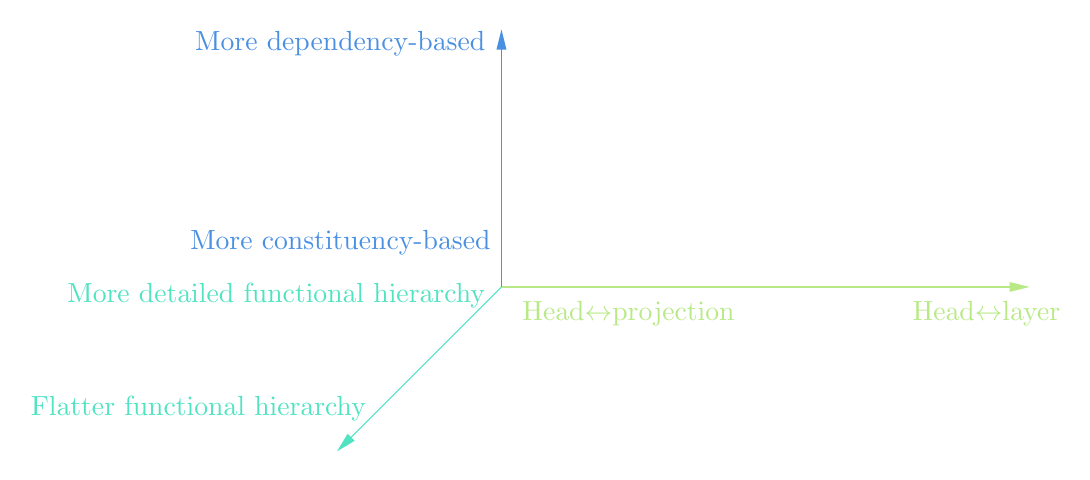
\begin{tikzpicture}[x=0.75pt,y=0.75pt,yscale=-0.8,xscale=0.8]
%uncomment if require: \path (0,536); %set diagram left start at 0, and has height of 536

%Straight Lines [id:da308608375613858] 
\draw [color={rgb, 255:red, 80; green, 227; blue, 194 }  ,draw opacity=1 ]   (323,220.81) -- (225.41,318.4) ;
\draw [shift={(224,319.81)}, rotate = 315] [fill={rgb, 255:red, 80; green, 227; blue, 194 }  ,fill opacity=1 ][line width=0.08]  [draw opacity=0] (12,-3) -- (0,0) -- (12,3) -- cycle    ;
%Straight Lines [id:da6591124487064512] 
\draw [color={rgb, 255:red, 184; green, 233; blue, 134 }  ,draw opacity=1 ]   (323,220.81) -- (639,220.81) ;
\draw [shift={(641,220.81)}, rotate = 180] [fill={rgb, 255:red, 184; green, 233; blue, 134 }  ,fill opacity=1 ][line width=0.08]  [draw opacity=0] (12,-3) -- (0,0) -- (12,3) -- cycle    ;
%Straight Lines [id:da7487030405468103] 
\draw [color={rgb, 255:red, 74; green, 144; blue, 226 }  ,draw opacity=1 ]   (323,220.81) -- (323,67.81) ;
\draw [shift={(323,65.81)}, rotate = 90] [fill={rgb, 255:red, 74; green, 144; blue, 226 }  ,fill opacity=1 ][line width=0.08]  [draw opacity=0] (12,-3) -- (0,0) -- (12,3) -- cycle    ;

% Text Node
\draw (137,65) node [anchor=north west][inner sep=0.75pt]  [color={rgb, 255:red, 74; green, 144; blue, 226 }  ,opacity=1 ] [align=left] {More dependency-based};
% Text Node
\draw (134,185) node [anchor=north west][inner sep=0.75pt]  [color={rgb, 255:red, 74; green, 144; blue, 226 }  ,opacity=1 ] [align=left] {More constituency-based};
% Text Node
\draw (60,217) node [anchor=north west][inner sep=0.75pt]  [color={rgb, 255:red, 80; green, 227; blue, 194 }  ,opacity=1 ] [align=left] {More detailed functional hierarchy};
% Text Node
\draw (38,285) node [anchor=north west][inner sep=0.75pt]  [color={rgb, 255:red, 80; green, 227; blue, 194 }  ,opacity=1 ] [align=left] {Flatter functional hierarchy};
% Text Node
\draw (334,228) node [anchor=north west][inner sep=0.75pt]  [color={rgb, 255:red, 184; green, 233; blue, 134 }  ,opacity=1 ] [align=left] {Head$\displaystyle \leftrightarrow $projection};
% Text Node
\draw (569,228) node [anchor=north west][inner sep=0.75pt]  [color={rgb, 255:red, 184; green, 233; blue, 134 }  ,opacity=1 ] [align=left] {Head$\displaystyle \leftrightarrow $layer};


\end{tikzpicture}

    \caption{Dimensions used to } % TODO:取一个适合的名字:Minimalism的各种等价描述的坐标轴?
\end{figure}

\subsubsection{Dependency vs constituency}

Dependency relations

\subsubsection{Divergent standards of constituency}

Note that in the above discussion, a word -- a bundle of several features spelt-out together -- is a \emph{span}
and not a constituent in the generative sense, and yet people recognize it as a construction. This % TODO

So now we can see there is no conflict between the binary branching definition of \emph{verb phrase} as Aux plus V plus NP_{\text{object}} and the \ac{blt} definition of verb phrase. A good choice is to use the term 
\emph{verb complex} to denote verb phrase in the \ac{blt} sense \citep{Wilbur2014}.

There is yet a final issue about how flat the syntax tree should be. % 说明这个讨论没啥意义:flat tree要求更多dependency relations

\subsubsection{The notion of \emph{head}}\label{sec:headedness}

What is the head of a phrase is also a topic causing lots of disputation. 

So here we see the root cause of the disagreement between Minimalism and the \ac{blt}- or \ac{cgel}-definition 
of head. The former is about labeling a newly introduced element (i.e. the specifier), while the latter is about 
the the overall syntactic function of the whole phrase. 

\subsubsection{Minimalism as constructivism}

\subsection{Deriving the diverse formalisms}

% TODO: linking MP, CGEL and dependency grammar

\subsubsection{Complements and modifiers}

It should be noted that the distinction between complements and modifiers are still opaque even with 
all these discussions about licensing and selection, and this opaqueness is theoretically rooted. 
Languages that have a relatively fixed word order often impose (though usually in a rather subtle way) 
a word order constraints on different types of clausal adjuncts and adjectives in NPs, 
which is well explained by the cartographic approach as we see above that the adjuncts and NP modifiers 
are actually introduced by a fixed hierarchy of functional heads. Since we consider the functional heads 
to be realized \emph{onto} the \ac{cgel} head of the construction -- the main noun, the main verb, etc. -- 
it follows that adjectives about different properties fill different ``slots of modifiers'' of the head noun, 
and similarly adjuncts about different properties fill different ``slots of modifiers'' of the head verb, 
in exactly the same way arguments fill argument slots. 

A clear distinction between complements and modifiers -- or in the cause of clause structure, arguments and
adjuncts -- is therefore of limited purely formal interest and is better viewed as a language-specific concept, 
which may be useful for description \citep{haspelmath2014arguments}. 

The \ac{cgel} approach of dependent types effectively gives us something like the good old X-bar theory, where a lexical word 
(not a functional word, especially not an invisible functional head) heads a phrase with multiple 
complements, specifiers and adjuncts (all in generative terms). The main differences between the GB-like 
X-bar scheme and the \ac{cgel} scheme are that in the former terms like ``complement'' is defined strictly 
in structural terms (e.g. ``the sister of the head''), while in the latter these terms are defined in 
terms of dependency relations (e.g. ``complements are more explicitly licensed by the head than 
modifiers'') without any guarantee that complements are necessarily lower than modifiers \citep{payne2007fusion},
and that in the \ac{cgel} framework there is no intermediate projections: nominals in \ac{cgel} corresponds 
to N' projections in X-bar theory, but the former can appear as a complete unit (e.g. as the modifier of another 
NP). 

We can summarize that the framework in \ac{cgel} is a little more flexible than X-bar theory. 
From the Minimalism perspective, it is easy to explain why: the criteria \ac{cgel} uses to draw the line 
between complements and modifiers are related more to spellout (see the discussion in \prettyref{sec:sub-cat})
than the tree structure, and therefore purely tree structure-based notion of ``complements'' is bond to fail. 
So-called intermediate projections in X-bar theory, like N', are actually maximal projections according to 
more fine-grained analysis, and hence they indeed can appear as a complete phrase.
The X-bar theory is therefore just a transitional version of generative syntax.

\subsubsection{Movements}

\subsubsection{Empty categories and fusion-function constructions}

\subsubsection{Feature structures}

\subsubsection{Selection and subcagegorization}\label{sec:sub-cat}

Another reason to keep pre-compiled trees is it makes the theory more psychologically plausible \citep{brain-syntax-1,brain-syntax-2}.

\subsection{Categories and the notion of ``word''}

A \concept{category}\index{category} is defined as a type of constructions with similar distributions.
I will first discuss basic syntactic constructions and identify positions that can be filled in them, 
and then search possible constructions in these positions. This is how categories can be recognized.

A construction that is small enough is said to be a \concept{word} or more precisely, 
a \concept{grammatical word}\index{word!grammatical}.
I emphasize \emph{grammatical} because it is quite common to use the term \emph{word} 词 to denote 
a \concept{prosody word}\index{word!prosody}. Prosody is important in Chinese, which is discussed in 
\prettyref{sec:prosody-intro} and \prettyref{chap:prosody-overview}. 

In traditional grammars concerning Latin, a common practice is to roughly define word classes (nouns, verbs, etc.) 
according to their meaning and then discuss where they can be used. 
In this proto-book I do not take this approach. Though I will review a lot of work based on the meaning-first 
approach, the way I distinguish word classes is mainly distributional. If two words can appear in similar
positions, they are classified into one \concept{word class}\index{word class} or \concept{part of speech}.
A word class is just a category about words.  

In other words, I define concepts like \emph{noun-like} and \emph{verb-like} \emph{before} listing criteria of 
what is a noun and what is a verb. Criteria for word classes are always language-specific, but we have more 
confidence that at least some \emph{features} -- like the nominal feature \textit{n} or the verbal feature 
\textit{v} -- are cross-linguistic and may be attributed to the language faculty in the broad sense. 

\section{The mixed framework}

% Predicator,NP等概念 argument structure 见syntax within the word一书

After length discussions, it is time to go back and summarize the framework I adopt in this proto-book.

Having worked out a \emph{formal} grammatical framework, a list of frequently met constructions 
are still required. Languages have both formal and substantial universals. The former is purely about 
how structures are built, while the latter is about what raw materials are fed into the structure 
building machine. 

% BLT, CGEL, 中比较实质性的概念

We use the term \concept{verb phrase (VP)} to denote % TODO: if there is V to T movement?

\section{Data sources}

% 关于语料来源和分析方法

\end{document}